\documentclass[a1paper,fleqn]{betterportraitposter}

% PACKAGES
\usepackage[none]{hyphenat}
\usepackage{lipsum}

\usepackage{tikz}
\usepackage{wrapfig}

%%%% Uncomment the following commands to customise the format

%% Setting the height of the top and bottom (colored) bars
%% Uncomment either of the following lines it you want to change the defaults heights of the top or bottom bars.
% \setlength{\mainfindingheight}{0.5\paperheight} % Top bar
% \setlength{\bottomboxheight}{0.10\paperheight} % Bottom bar

%% Setting the page margin

%% Changing font sizes
% Text font
%\renewcommand{\fontsizestandard}{\fontsize{28}{35} \selectfont}
% Main column font
%\renewcommand{\fontsizemain}{\fontsize{28}{35} \selectfont}
% Title font
%\renewcommand{\fontsizetitle}{\fontsize{28}{35} \selectfont}
% Author font
%\renewcommand{\fontsizeauthor}{\fontsize{28}{35} \selectfont}
% Institution font
%\renewcommand{\fontsizeauthor}{\fontsize{28}{35} \selectfont}
% Section font
%\renewcommand{\fontsizesection}{\fontsize{28}{35} \selectfont}

%% Changing font sizes for a specific text segment
% Place the text inside brackets:
% {\fontsize{28}{35} \selectfont Your text goes here}

%% Changing colours
% Background of main claim box (options include: imperialblue, empirical, theory, methods and intervention
% Default is empirical
% \renewcommand{\maincolumnbackgroundcolor}{intervention}

% Font on main and bottom boxes
% \renewcommand{\maincolumnfontcolor}{empirical}

\definecolor{mygray}{RGB}{66, 66, 65}
\definecolor{myblue}{RGB}{0, 79, 159}
\renewcommand{\maincolumnbackgroundcolor}{mygray}

\renewcommand{\emph}[1]{\textbf{\color{myblue}#1}}

%%%%% NEW MATH DEFINITIONS %%%%%

\usepackage{amsmath,amsfonts,bm}

% Mark sections of captions for referring to divisions of figures
\newcommand{\figleft}{{\em (Left)}}
\newcommand{\figcenter}{{\em (Center)}}
\newcommand{\figright}{{\em (Right)}}
\newcommand{\figtop}{{\em (Top)}}
\newcommand{\figbottom}{{\em (Bottom)}}
\newcommand{\captiona}{{\em (a)}}
\newcommand{\captionb}{{\em (b)}}
\newcommand{\captionc}{{\em (c)}}
\newcommand{\captiond}{{\em (d)}}

% Highlight a newly defined term
\newcommand{\newterm}[1]{{\bf #1}}


% Figure reference, lower-case.
\def\figref#1{Figure~\ref{#1}}
% Figure reference, capital. For start of sentence
\def\Figref#1{Figure~\ref{#1}}
\def\twofigref#1#2{figures \ref{#1} and \ref{#2}}
\def\quadfigref#1#2#3#4{figures \ref{#1}, \ref{#2}, \ref{#3} and \ref{#4}}
% Section reference, lower-case.
\def\secref#1{section~\ref{#1}}
% Section reference, capital.
\def\Secref#1{Section~\ref{#1}}
% Reference to two sections.
\def\twosecrefs#1#2{sections \ref{#1} and \ref{#2}}
% Reference to three sections.
\def\secrefs#1#2#3{sections \ref{#1}, \ref{#2} and \ref{#3}}
% Reference to an equation, lower-case.
% \def\eqref#1{\eqref{#1}}
% Reference to an equation, upper case
% \def\Eqref#1{Equation~\ref{#1}}
% A raw reference to an equation---avoid using if possible
\def\plaineqref#1{\ref{#1}}
% Reference to a chapter, lower-case.
\def\chapref#1{chapter~\ref{#1}}
% Reference to an equation, upper case.
\def\Chapref#1{Chapter~\ref{#1}}
% Reference to a range of chapters
\def\rangechapref#1#2{chapters\ref{#1}--\ref{#2}}
% Reference to an algorithm, lower-case.
\def\algref#1{algorithm~\ref{#1}}
% Reference to an algorithm, upper case.
\def\Algref#1{Algorithm~\ref{#1}}
\def\twoalgref#1#2{algorithms \ref{#1} and \ref{#2}}
\def\Twoalgref#1#2{Algorithms \ref{#1} and \ref{#2}}
% Reference to a part, lower case
\def\partref#1{part~\ref{#1}}
% Reference to a part, upper case
\def\Partref#1{Part~\ref{#1}}
\def\twopartref#1#2{parts \ref{#1} and \ref{#2}}

\def\ceil#1{\lceil #1 \rceil}
\def\floor#1{\lfloor #1 \rfloor}
\def\1{\bm{1}}
\newcommand{\train}{\mathcal{D}}
\newcommand{\valid}{\mathcal{D_{\mathrm{valid}}}}
\newcommand{\test}{\mathcal{D_{\mathrm{test}}}}

\def\eps{{\epsilon}}


% Random variables
\def\reta{{\textnormal{$\eta$}}}
\def\ra{{\textnormal{a}}}
\def\rb{{\textnormal{b}}}
\def\rc{{\textnormal{c}}}
\def\rd{{\textnormal{d}}}
\def\re{{\textnormal{e}}}
\def\rf{{\textnormal{f}}}
\def\rg{{\textnormal{g}}}
\def\rh{{\textnormal{h}}}
\def\ri{{\textnormal{i}}}
\def\rj{{\textnormal{j}}}
\def\rk{{\textnormal{k}}}
\def\rl{{\textnormal{l}}}
% rm is already a command, just don't name any random variables m
\def\rn{{\textnormal{n}}}
\def\ro{{\textnormal{o}}}
\def\rp{{\textnormal{p}}}
\def\rq{{\textnormal{q}}}
\def\rr{{\textnormal{r}}}
\def\rs{{\textnormal{s}}}
\def\rt{{\textnormal{t}}}
\def\ru{{\textnormal{u}}}
\def\rv{{\textnormal{v}}}
\def\rw{{\textnormal{w}}}
\def\rx{{\textnormal{x}}}
\def\ry{{\textnormal{y}}}
\def\rz{{\textnormal{z}}}

% Random vectors
\def\rvepsilon{{\mathbf{\epsilon}}}
\def\rvtheta{{\mathbf{\theta}}}
\def\rva{{\mathbf{a}}}
\def\rvb{{\mathbf{b}}}
\def\rvc{{\mathbf{c}}}
\def\rvd{{\mathbf{d}}}
\def\rve{{\mathbf{e}}}
\def\rvf{{\mathbf{f}}}
\def\rvg{{\mathbf{g}}}
\def\rvh{{\mathbf{h}}}
\def\rvu{{\mathbf{i}}}
\def\rvj{{\mathbf{j}}}
\def\rvk{{\mathbf{k}}}
\def\rvl{{\mathbf{l}}}
\def\rvm{{\mathbf{m}}}
\def\rvn{{\mathbf{n}}}
\def\rvo{{\mathbf{o}}}
\def\rvp{{\mathbf{p}}}
\def\rvq{{\mathbf{q}}}
\def\rvr{{\mathbf{r}}}
\def\rvs{{\mathbf{s}}}
\def\rvt{{\mathbf{t}}}
\def\rvu{{\mathbf{u}}}
\def\rvv{{\mathbf{v}}}
\def\rvw{{\mathbf{w}}}
\def\rvx{{\mathbf{x}}}
\def\rvy{{\mathbf{y}}}
\def\rvz{{\mathbf{z}}}
\def\rvzeta{{\mathbf{\zeta}}}

% Elements of random vectors
\def\erva{{\textnormal{a}}}
\def\ervb{{\textnormal{b}}}
\def\ervc{{\textnormal{c}}}
\def\ervd{{\textnormal{d}}}
\def\erve{{\textnormal{e}}}
\def\ervf{{\textnormal{f}}}
\def\ervg{{\textnormal{g}}}
\def\ervh{{\textnormal{h}}}
\def\ervi{{\textnormal{i}}}
\def\ervj{{\textnormal{j}}}
\def\ervk{{\textnormal{k}}}
\def\ervl{{\textnormal{l}}}
\def\ervm{{\textnormal{m}}}
\def\ervn{{\textnormal{n}}}
\def\ervo{{\textnormal{o}}}
\def\ervp{{\textnormal{p}}}
\def\ervq{{\textnormal{q}}}
\def\ervr{{\textnormal{r}}}
\def\ervs{{\textnormal{s}}}
\def\ervt{{\textnormal{t}}}
\def\ervu{{\textnormal{u}}}
\def\ervv{{\textnormal{v}}}
\def\ervw{{\textnormal{w}}}
\def\ervx{{\textnormal{x}}}
\def\ervy{{\textnormal{y}}}
\def\ervz{{\textnormal{z}}}

% Random matrices
\def\rmA{{\mathbf{A}}}
\def\rmB{{\mathbf{B}}}
\def\rmC{{\mathbf{C}}}
\def\rmD{{\mathbf{D}}}
\def\rmE{{\mathbf{E}}}
\def\rmF{{\mathbf{F}}}
\def\rmG{{\mathbf{G}}}
\def\rmH{{\mathbf{H}}}
\def\rmI{{\mathbf{I}}}
\def\rmJ{{\mathbf{J}}}
\def\rmK{{\mathbf{K}}}
\def\rmL{{\mathbf{L}}}
\def\rmM{{\mathbf{M}}}
\def\rmN{{\mathbf{N}}}
\def\rmO{{\mathbf{O}}}
\def\rmP{{\mathbf{P}}}
\def\rmQ{{\mathbf{Q}}}
\def\rmR{{\mathbf{R}}}
\def\rmS{{\mathbf{S}}}
\def\rmT{{\mathbf{T}}}
\def\rmU{{\mathbf{U}}}
\def\rmV{{\mathbf{V}}}
\def\rmW{{\mathbf{W}}}
\def\rmX{{\mathbf{X}}}
\def\rmY{{\mathbf{Y}}}
\def\rmZ{{\mathbf{Z}}}

% Elements of random matrices
\def\ermA{{\textnormal{A}}}
\def\ermB{{\textnormal{B}}}
\def\ermC{{\textnormal{C}}}
\def\ermD{{\textnormal{D}}}
\def\ermE{{\textnormal{E}}}
\def\ermF{{\textnormal{F}}}
\def\ermG{{\textnormal{G}}}
\def\ermH{{\textnormal{H}}}
\def\ermI{{\textnormal{I}}}
\def\ermJ{{\textnormal{J}}}
\def\ermK{{\textnormal{K}}}
\def\ermL{{\textnormal{L}}}
\def\ermM{{\textnormal{M}}}
\def\ermN{{\textnormal{N}}}
\def\ermO{{\textnormal{O}}}
\def\ermP{{\textnormal{P}}}
\def\ermQ{{\textnormal{Q}}}
\def\ermR{{\textnormal{R}}}
\def\ermS{{\textnormal{S}}}
\def\ermT{{\textnormal{T}}}
\def\ermU{{\textnormal{U}}}
\def\ermV{{\textnormal{V}}}
\def\ermW{{\textnormal{W}}}
\def\ermX{{\textnormal{X}}}
\def\ermY{{\textnormal{Y}}}
\def\ermZ{{\textnormal{Z}}}

% Vectors
\def\vzero{{\bm{0}}}
\def\vone{{\bm{1}}}
\def\vmu{{\bm{\mu}}}
\def\vtheta{{\bm{\theta}}}
\def\va{{\bm{a}}}
\def\vb{{\bm{b}}}
\def\vc{{\bm{c}}}
\def\vd{{\bm{d}}}
\def\ve{{\bm{e}}}
\def\vf{{\bm{f}}}
\def\vg{{\bm{g}}}
\def\vh{{\bm{h}}}
\def\vi{{\bm{i}}}
\def\vj{{\bm{j}}}
\def\vk{{\bm{k}}}
\def\vl{{\bm{l}}}
\def\vm{{\bm{m}}}
\def\vn{{\bm{n}}}
\def\vo{{\bm{o}}}
\def\vp{{\bm{p}}}
\def\vq{{\bm{q}}}
\def\vr{{\bm{r}}}
\def\vs{{\bm{s}}}
\def\vt{{\bm{t}}}
\def\vu{{\bm{u}}}
\def\vv{{\bm{v}}}
\def\vw{{\bm{w}}}
\def\vx{{\bm{x}}}
\def\vy{{\bm{y}}}
\def\vz{{\bm{z}}}

% Elements of vectors
\def\evalpha{{\alpha}}
\def\evbeta{{\beta}}
\def\evepsilon{{\epsilon}}
\def\evlambda{{\lambda}}
\def\evomega{{\omega}}
\def\evmu{{\mu}}
\def\evpsi{{\psi}}
\def\evsigma{{\sigma}}
\def\evtheta{{\theta}}
\def\eva{{a}}
\def\evb{{b}}
\def\evc{{c}}
\def\evd{{d}}
\def\eve{{e}}
\def\evf{{f}}
\def\evg{{g}}
\def\evh{{h}}
\def\evi{{i}}
\def\evj{{j}}
\def\evk{{k}}
\def\evl{{l}}
\def\evm{{m}}
\def\evn{{n}}
\def\evo{{o}}
\def\evp{{p}}
\def\evq{{q}}
\def\evr{{r}}
\def\evs{{s}}
\def\evt{{t}}
\def\evu{{u}}
\def\evv{{v}}
\def\evw{{w}}
\def\evx{{x}}
\def\evy{{y}}
\def\evz{{z}}

% Matrix
\def\mA{{\bm{A}}}
\def\mB{{\bm{B}}}
\def\mC{{\bm{C}}}
\def\mD{{\bm{D}}}
\def\mE{{\bm{E}}}
\def\mF{{\bm{F}}}
\def\mG{{\bm{G}}}
\def\mH{{\bm{H}}}
\def\mI{{\bm{I}}}
\def\mJ{{\bm{J}}}
\def\mK{{\bm{K}}}
\def\mL{{\bm{L}}}
\def\mM{{\bm{M}}}
\def\mN{{\bm{N}}}
\def\mO{{\bm{O}}}
\def\mP{{\bm{P}}}
\def\mQ{{\bm{Q}}}
\def\mR{{\bm{R}}}
\def\mS{{\bm{S}}}
\def\mT{{\bm{T}}}
\def\mU{{\bm{U}}}
\def\mV{{\bm{V}}}
\def\mW{{\bm{W}}}
\def\mX{{\bm{X}}}
\def\mY{{\bm{Y}}}
\def\mZ{{\bm{Z}}}
\def\mBeta{{\bm{\beta}}}
\def\mPhi{{\bm{\Phi}}}
\def\mLambda{{\bm{\Lambda}}}
\def\mSigma{{\bm{\Sigma}}}

% Tensor
\DeclareMathAlphabet{\mathsfit}{\encodingdefault}{\sfdefault}{m}{sl}
\SetMathAlphabet{\mathsfit}{bold}{\encodingdefault}{\sfdefault}{bx}{n}
\newcommand{\tens}[1]{\bm{\mathsfit{#1}}}
\def\tA{{\tens{A}}}
\def\tB{{\tens{B}}}
\def\tC{{\tens{C}}}
\def\tD{{\tens{D}}}
\def\tE{{\tens{E}}}
\def\tF{{\tens{F}}}
\def\tG{{\tens{G}}}
\def\tH{{\tens{H}}}
\def\tI{{\tens{I}}}
\def\tJ{{\tens{J}}}
\def\tK{{\tens{K}}}
\def\tL{{\tens{L}}}
\def\tM{{\tens{M}}}
\def\tN{{\tens{N}}}
\def\tO{{\tens{O}}}
\def\tP{{\tens{P}}}
\def\tQ{{\tens{Q}}}
\def\tR{{\tens{R}}}
\def\tS{{\tens{S}}}
\def\tT{{\tens{T}}}
\def\tU{{\tens{U}}}
\def\tV{{\tens{V}}}
\def\tW{{\tens{W}}}
\def\tX{{\tens{X}}}
\def\tY{{\tens{Y}}}
\def\tZ{{\tens{Z}}}


% Graph
\def\gA{{\mathcal{A}}}
\def\gB{{\mathcal{B}}}
\def\gC{{\mathcal{C}}}
\def\gD{{\mathcal{D}}}
\def\gE{{\mathcal{E}}}
\def\gF{{\mathcal{F}}}
\def\gG{{\mathcal{G}}}
\def\gH{{\mathcal{H}}}
\def\gI{{\mathcal{I}}}
\def\gJ{{\mathcal{J}}}
\def\gK{{\mathcal{K}}}
\def\gL{{\mathcal{L}}}
\def\gM{{\mathcal{M}}}
\def\gN{{\mathcal{N}}}
\def\gO{{\mathcal{O}}}
\def\gP{{\mathcal{P}}}
\def\gQ{{\mathcal{Q}}}
\def\gR{{\mathcal{R}}}
\def\gS{{\mathcal{S}}}
\def\gT{{\mathcal{T}}}
\def\gU{{\mathcal{U}}}
\def\gV{{\mathcal{V}}}
\def\gW{{\mathcal{W}}}
\def\gX{{\mathcal{X}}}
\def\gY{{\mathcal{Y}}}
\def\gZ{{\mathcal{Z}}}

% Sets
\def\sA{{\mathbb{A}}}
\def\sB{{\mathbb{B}}}
\def\sC{{\mathbb{C}}}
\def\sD{{\mathbb{D}}}
% Don't use a set called E, because this would be the same as our symbol
% for expectation.
\def\sF{{\mathbb{F}}}
\def\sG{{\mathbb{G}}}
\def\sH{{\mathbb{H}}}
\def\sI{{\mathbb{I}}}
\def\sJ{{\mathbb{J}}}
\def\sK{{\mathbb{K}}}
\def\sL{{\mathbb{L}}}
\def\sM{{\mathbb{M}}}
\def\sN{{\mathbb{N}}}
\def\sO{{\mathbb{O}}}
\def\sP{{\mathbb{P}}}
\def\sQ{{\mathbb{Q}}}
\def\sR{{\mathbb{R}}}
\def\sS{{\mathbb{S}}}
\def\sT{{\mathbb{T}}}
\def\sU{{\mathbb{U}}}
\def\sV{{\mathbb{V}}}
\def\sW{{\mathbb{W}}}
\def\sX{{\mathbb{X}}}
\def\sY{{\mathbb{Y}}}
\def\sZ{{\mathbb{Z}}}

% Entries of a matrix
\def\emLambda{{\Lambda}}
\def\emA{{A}}
\def\emB{{B}}
\def\emC{{C}}
\def\emD{{D}}
\def\emE{{E}}
\def\emF{{F}}
\def\emG{{G}}
\def\emH{{H}}
\def\emI{{I}}
\def\emJ{{J}}
\def\emK{{K}}
\def\emL{{L}}
\def\emM{{M}}
\def\emN{{N}}
\def\emO{{O}}
\def\emP{{P}}
\def\emQ{{Q}}
\def\emR{{R}}
\def\emS{{S}}
\def\emT{{T}}
\def\emU{{U}}
\def\emV{{V}}
\def\emW{{W}}
\def\emX{{X}}
\def\emY{{Y}}
\def\emZ{{Z}}
\def\emSigma{{\Sigma}}

% entries of a tensor
% Same font as tensor, without \bm wrapper
\newcommand{\etens}[1]{\mathsfit{#1}}
\def\etLambda{{\etens{\Lambda}}}
\def\etA{{\etens{A}}}
\def\etB{{\etens{B}}}
\def\etC{{\etens{C}}}
\def\etD{{\etens{D}}}
\def\etE{{\etens{E}}}
\def\etF{{\etens{F}}}
\def\etG{{\etens{G}}}
\def\etH{{\etens{H}}}
\def\etI{{\etens{I}}}
\def\etJ{{\etens{J}}}
\def\etK{{\etens{K}}}
\def\etL{{\etens{L}}}
\def\etM{{\etens{M}}}
\def\etN{{\etens{N}}}
\def\etO{{\etens{O}}}
\def\etP{{\etens{P}}}
\def\etQ{{\etens{Q}}}
\def\etR{{\etens{R}}}
\def\etS{{\etens{S}}}
\def\etT{{\etens{T}}}
\def\etU{{\etens{U}}}
\def\etV{{\etens{V}}}
\def\etW{{\etens{W}}}
\def\etX{{\etens{X}}}
\def\etY{{\etens{Y}}}
\def\etZ{{\etens{Z}}}

% The true underlying data generating distribution
\newcommand{\pdata}{p_{\rm{data}}}
% The empirical distribution defined by the training set
\newcommand{\ptrain}{\hat{p}_{\rm{data}}}
\newcommand{\Ptrain}{\hat{P}_{\rm{data}}}
% The model distribution
\newcommand{\pmodel}{p_{\rm{model}}}
\newcommand{\Pmodel}{P_{\rm{model}}}
\newcommand{\ptildemodel}{\tilde{p}_{\rm{model}}}
% Stochastic autoencoder distributions
\newcommand{\pencode}{p_{\rm{encoder}}}
\newcommand{\pdecode}{p_{\rm{decoder}}}
\newcommand{\precons}{p_{\rm{reconstruct}}}

\newcommand{\laplace}{\mathrm{Laplace}} % Laplace distribution

\newcommand{\E}{\mathbb{E}}
\newcommand{\Ls}{\mathcal{L}}
\newcommand{\R}{\mathbb{R}}
\newcommand{\emp}{\tilde{p}}
\newcommand{\lr}{\alpha}
\newcommand{\reg}{\lambda}
\newcommand{\rect}{\mathrm{rectifier}}
\newcommand{\softmax}{\mathrm{softmax}}
\newcommand{\sigmoid}{\sigma}
\newcommand{\softplus}{\zeta}
\newcommand{\KL}{D_{\mathrm{KL}}}
\newcommand{\Var}{\mathrm{Var}}
\newcommand{\standarderror}{\mathrm{SE}}
\newcommand{\Cov}{\mathrm{Cov}}
% Wolfram Mathworld says $L^2$ is for function spaces and $\ell^2$ is for vectors
% But then they seem to use $L^2$ for vectors throughout the site, and so does
% wikipedia.
\newcommand{\normlzero}{L^0}
\newcommand{\normlone}{L^1}
\newcommand{\normltwo}{L^2}
\newcommand{\normlp}{L^p}
\newcommand{\normmax}{L^\infty}

\newcommand{\parents}{Pa} % See usage in notation.tex. Chosen to match Daphne's book.

\DeclareMathOperator*{\argmax}{arg\,max}
\DeclareMathOperator*{\argmin}{arg\,min}

\DeclareMathOperator{\sign}{sign}
\DeclareMathOperator{\Tr}{Tr}
\let\ab\allowbreak

% custom commands
% \newcommand{\R}{\mathbb{R}}
\newcommand{\N}{\mathbb{N}}
\renewcommand{\P}{\mathbb{P}}
\newcommand{\C}{\mathcal{C}}
\renewcommand{\L}{\mathrm{L}}
\newcommand{\dx}{\mathrm{d}}
\newcommand{\X}{\mathcal{X}}
\newcommand{\Z}{\mathcal{Z}}
\newcommand{\T}{\mathcal{T}}
\newcommand{\id}{\mathrm{Id}}
\newcommand{\norm}[1]{\left\Vert#1\right\Vert}
\newcommand{\scal}[2]{\left\langle#1,#2\right\rangle}
\renewcommand{\vec}[1]{\mathbf{#1}}
\newcommand{\diameter}{\mathrm{diam}}
\newcommand{\prox}{\mathrm{prox}}
\newcommand{\proj}{\mathrm{proj}}
\newcommand{\tmin}{t_\mathrm{min}}
\newcommand{\tmax}{t_\mathrm{max}}
% \newcommand{\hatt}{\widehat{t}}
\def\hatt{{\widehat{t}}}
\newcommand{\tminh}{\hatt_\mathrm{min}}
\newcommand{\tmaxh}{\hatt_\mathrm{max}}

% \newcommand{\E}{\mathbb{E}}
\newcommand{\dist}[1]{\mathcal{P}_{#1}}
\newcommand{\pdf}[1]{p_{#1}}
\newcommand{\g}{\vert}
\newcommand{\normal}{\mathcal{N}}

\newcommand{\VP}{\mathrm{VP}}
\newcommand{\VE}{\mathrm{VE}}

\usepackage{amsmath}
\usepackage{amssymb}
\usepackage{mathtools}
\usepackage{amsthm}

\theoremstyle{plain}
\newtheorem{theorem}{Theorem}
% \newtheorem{proposition}[theorem]{Proposition}
% \newtheorem{lemma}[theorem]{Lemma}
% \newtheorem{corollary}[theorem]{Corollary}
% \theoremstyle{definition}
% \newtheorem{definition}[theorem]{Definition}
% \newtheorem{assumption}[theorem]{Assumption}
% \theoremstyle{remark}
% \newtheorem{remark}[theorem]{Remark}


\begin{document}	

%% Top box with main message
\mainfinding{\textbf{Denoising Score Matching Image Priors}}


%% Title, author and affiliations section
\titlebox{
    \title{}  
    \author{Erich Kobler$^\ast$ and Thomas Pock$^\dagger$ \\
    {\LARGE
    $^\ast$Department of Neuroradiology, University Hospital Bonn (\texttt{erich.kobler@ukbonn.de}) \hspace{1em} $^\dagger$Institute of Computer Graphics and Vision, Graz University of Technology 
    }}
}
% End of title stuff
    
    
%% Central box with traditional content
\centerbox{
{\fontsizesection\textbf{Abstract}\hspace*{1em}}
Recently, denoising score matching (DSM) and denoising diffusion-based (DD) models yielded remarkable results in imaging sciences.
These models are trained to approximate the gradient of the logarithmic data density perturbed by additive Gaussian noise, which results in smoother and more convex densities for increasing noise variance.
Thus, these models learn a graduated non-convexity heuristic.
To further exploit this effect, we propose DSM image priors that are learned on the joint density of (noisy) images and associated variance using score matching.
Facilitating these priors in the variational approach to inverse problems enables efficient optimization strategies -- even joint optimization w.r.t.~image and variance.
Moreover, learning the variance schedule of an unrolled proximal gradient scheme for specific tasks results in variational networks.


\begin{multicols}{2}
\section{A Graduated Non-convexity View of DSM-based Models}
Let~$\X\subset\R^d$ be bounded and consider a dataset of samples~$\{\vx_i\}_{i=1}^n\subset\X$ from the true data distribution~$\dist{\rvx}$ with density~$\pdf{\rvx}$.
Both noise-conditional score matching~(NCSM) and denoising diffusion probabilistic models~(DDPM) consider a smoothed data density
% The conditioning is either directly on the variance (NCSM) or a diffusion time (DDPM), encoding the variance.
% For simplicity we further assume the first case.
% Then, the conditional density of the perturbed noisy data reads as
\begin{align*}
\pdf{\rvx\vert\rt}(\vx\vert t) &= \left(\pdf{\rvx}\ast G(\vec{0},t\id)\right)(\vx)\propto \E_{\widehat{\vx}\sim\dist{\rvx}}\left[\exp\left(-\tfrac{\norm{\widehat{\vx}-\vx}_2^2}{2 t}\right)\right]
\end{align*}
and train neural networks~$S$ to predict the score, i.e., $S(\vx,t)\approx\nabla_\vx\log\pdf{\rvx\vert\rt}(\vx,t)$.\\[-.5em]

\textbf{Observe:}
Although the data becomes noisier with \emph{increasing variance}~$t$, the corresponding smooth probability density~$\pdf{\rvx\vert\rt}$ gets \emph{smoother} and its associated energy~$F(\vx,t)=-\log\pdf{\rvx\vert\rt}(\vx\vert t)$ gets more \emph{convex}.\\[-1em]

\begin{theorem}
Assuming~$\diameter(\X)<\infty$ and consindering $\pdf{}=\frac{1}{n}\sum_{i=1}^n \delta_{\vx_i}$, there exists a~$\widetilde{t}\in(0,\infty)$ such that the smoothed energy
\[
F(\vx,t)\coloneqq -\log \big( (p \ast G(\vec{0}, t\id))(\vx)\big)
\]
is convex w.r.t.~$\vx$ for all~$t\geq\widetilde{t}$.
\end{theorem}

Thus, the energy~$F(\vx,t)$ becomes easier to optimize for increasing~$t$.
This principle has already been exploited by the \emph{graduated non-convexity} heuristic:
\begin{enumerate}
\item Approximate true energy by one-parameter family~$F(\vx,t)$ for~$t\to0$
\item Choose initial~$t_0$ such that $F(\cdot,t_0)$ convex and decreasing sequence~$\{t_i\}_{i=1}^I$
\item Repeat for $i=1,2,\ldots,I$
\[
    \vx_i \approx \argmin_\vx F(\vx,t_i) \text{ starting from } \vx_{i-1}
\]
\end{enumerate}

\textbf{Observe:}
If a \emph{single gradient step} is performed in 3., this is equivalent to the \emph{denoising diffusion implicit model}~(DDIM) sampling without diffusion.

\vspace*{1em}
\textbf{Example:}
Find global minimum of a Gaussian mixture model~(GMM) using graduated non-convexity heuristic:

\noindent\begin{minipage}{.55\linewidth}
    \centering
    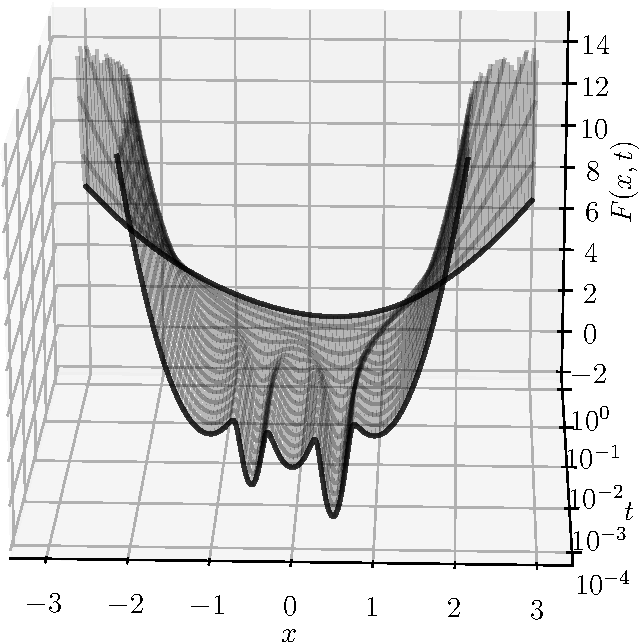
\includegraphics[width=.99\linewidth]{../figures/ex_gmm/ex_gmm_func}
\end{minipage}%
\noindent\begin{minipage}{.45\linewidth}
    \centering
    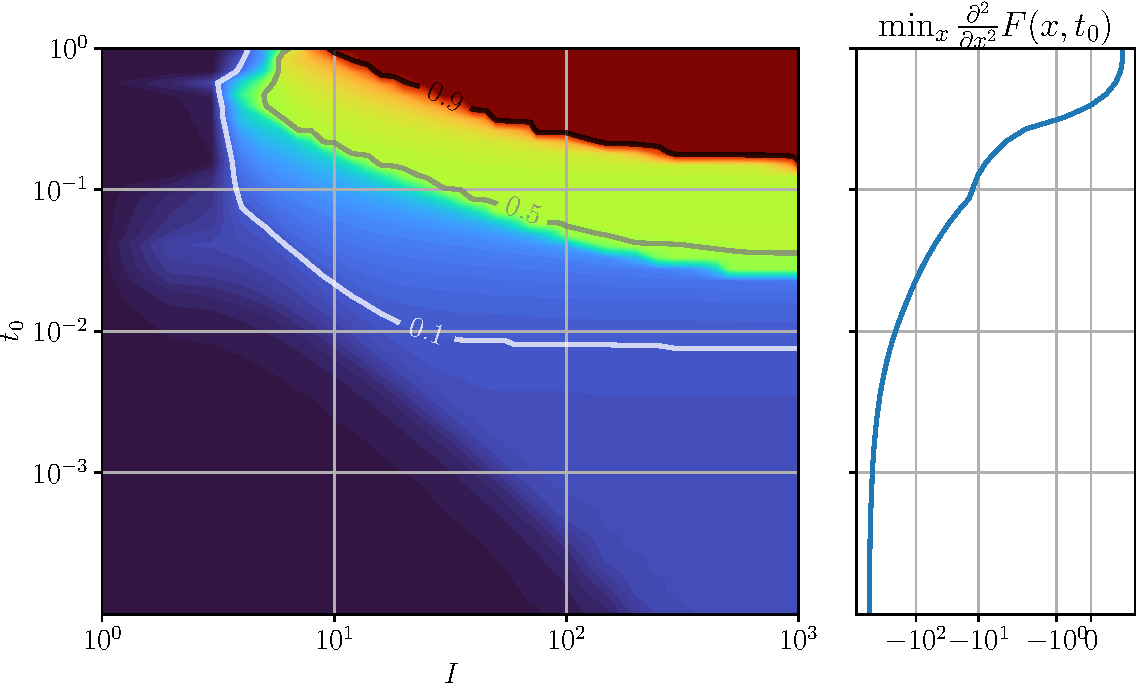
\includegraphics[width=.99\linewidth]{../figures/ex_gmm/ex_gmm_rate}
\end{minipage}
\begin{spacing}{1}
\LARGE
\LARGE
Left: Associated energy~$F(x,t)=-\log\pdf{}(x,t)$. Right top: Rate of start points~$x_0\in[-3,3]$ converging to the global minimum for different initial~$t_0$ and number of iterations~$I$. Right bottom: Illustration of minimal second derivative of~$F(x,t)$ for $x\in[-3,3]$.
\end{spacing}
\columnbreak

\section{Learning DSM Image Priors}
To extend the popular fields of experts image prior to the joint space of images~$\vx$ and variances~$t$, its energy is modeled by alternating convolution operators~$K_j$ and parametric 2D spline activation function~$\Phi_j$, i.e.
\[
R_L(\vx,t) = \scal{\vec{1}}{\left(\Phi_L(\cdot,t)\circ K_L\circ\cdots\circ\Phi_1(\cdot, t) \circ K_1\right)(\vx)}.
\]
To learn parameters of~$R_L$, we perform score matching on the joint density~$\dist{X,T}$:
\[
J_\mathrm{SM}(\theta)=\E_{\vx,t\sim\dist{\rvx,\rt}}\left[\tfrac12\norm{\nabla R_L(\vx,t;\theta) -\left(- \nabla\log p_{\rvx,\rt}(\vx,\rt)\right)}_M^2\right].
\]
By applying \emph{DSM for~$\vx$} and \emph{implicit score matching for~$t$} and using the logarithmic reparametrization~$\widehat{t}=\log t$ as well as $\vx=\widehat{\vx}+\exp(\tfrac{\widehat{t}}{2})\vn$, we get
\begin{align*}    
J(\theta)=\E_{\widehat{\vx},\vn,\widehat{t}\sim\dist{\widehat{\rvx},\rvn,\widehat{\rt}}}\tfrac12\Bigg[&\norm{e^{\widehat{t}/2}\nabla_\vx R_L(\vx,\widehat{t};\theta) -\vn}_2^2+\\
&m_t\left(\left(\tfrac{\partial}{\partial\widehat{t}}R_L(\vx,\widehat{t};\theta)\right)^2 -2\tfrac{\partial^2}{\partial \widehat{t}^2}R_L(\vx,\widehat{t};\theta)\right)\Bigg].
\end{align*}
This loss \emph{favors} prior energies~$R_L$ that \emph{slowly change} in the direction of~$t$ and are preferably \emph{convex}, which are desirable properties for optimization.
Moreover, the implicit score matching of~$\widehat{t}$ implements a data-driven regularization technique. 
\vspace*{-1em}
\begin{center}
\begin{tikzpicture}[every node/.append style={inner sep=1mm}, label/.style={draw=black,fill=white, inner sep=.5ex,rounded corners=1ex}]

\node[anchor=south] (r1) at (0,0) {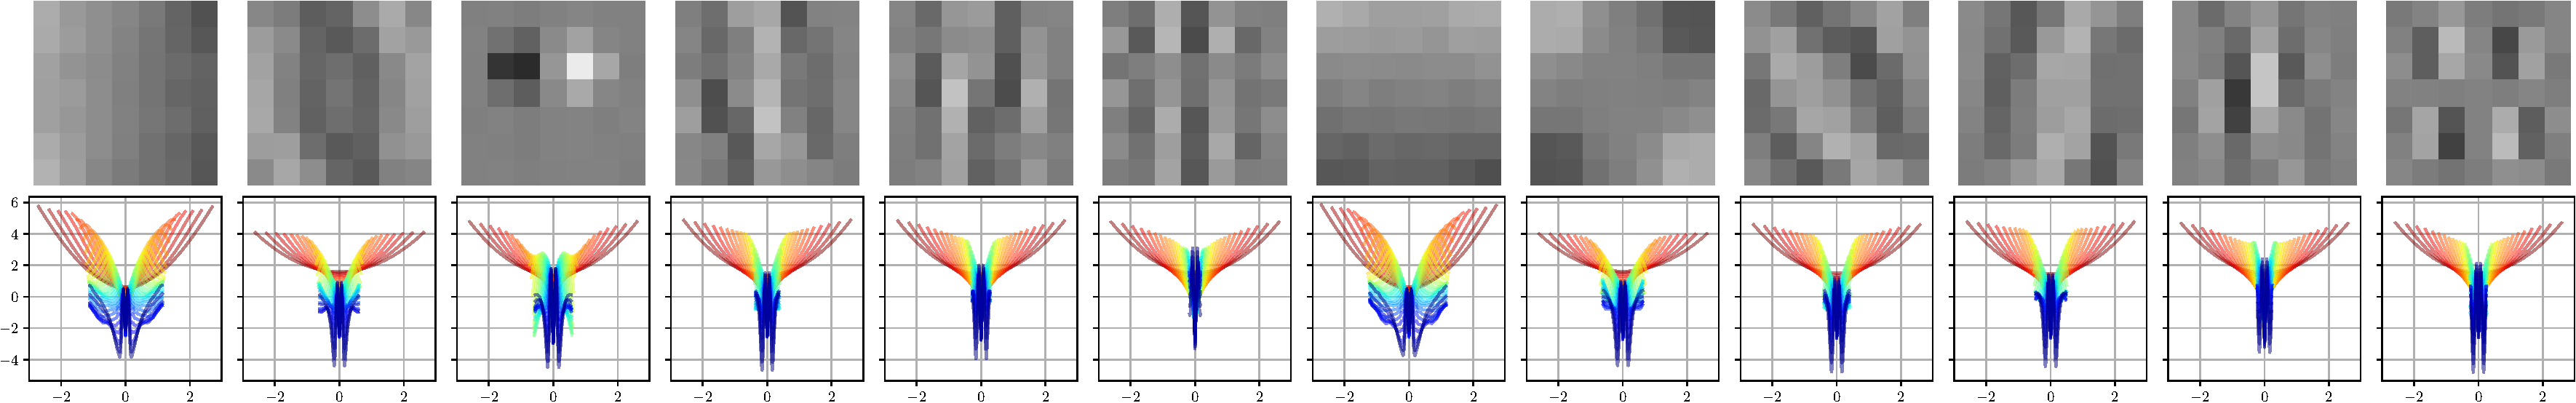
\includegraphics[width=.96\linewidth]{../figures/results/params_foe}};
\draw[black, very thick, rounded corners] (r1.north east) -- (r1.north west) -- (r1.south west) -- (r1.south east) node[midway,label,yshift=-1.25mm] {$R_1$};

\node[anchor=south] (r2) at (0,-9.5) {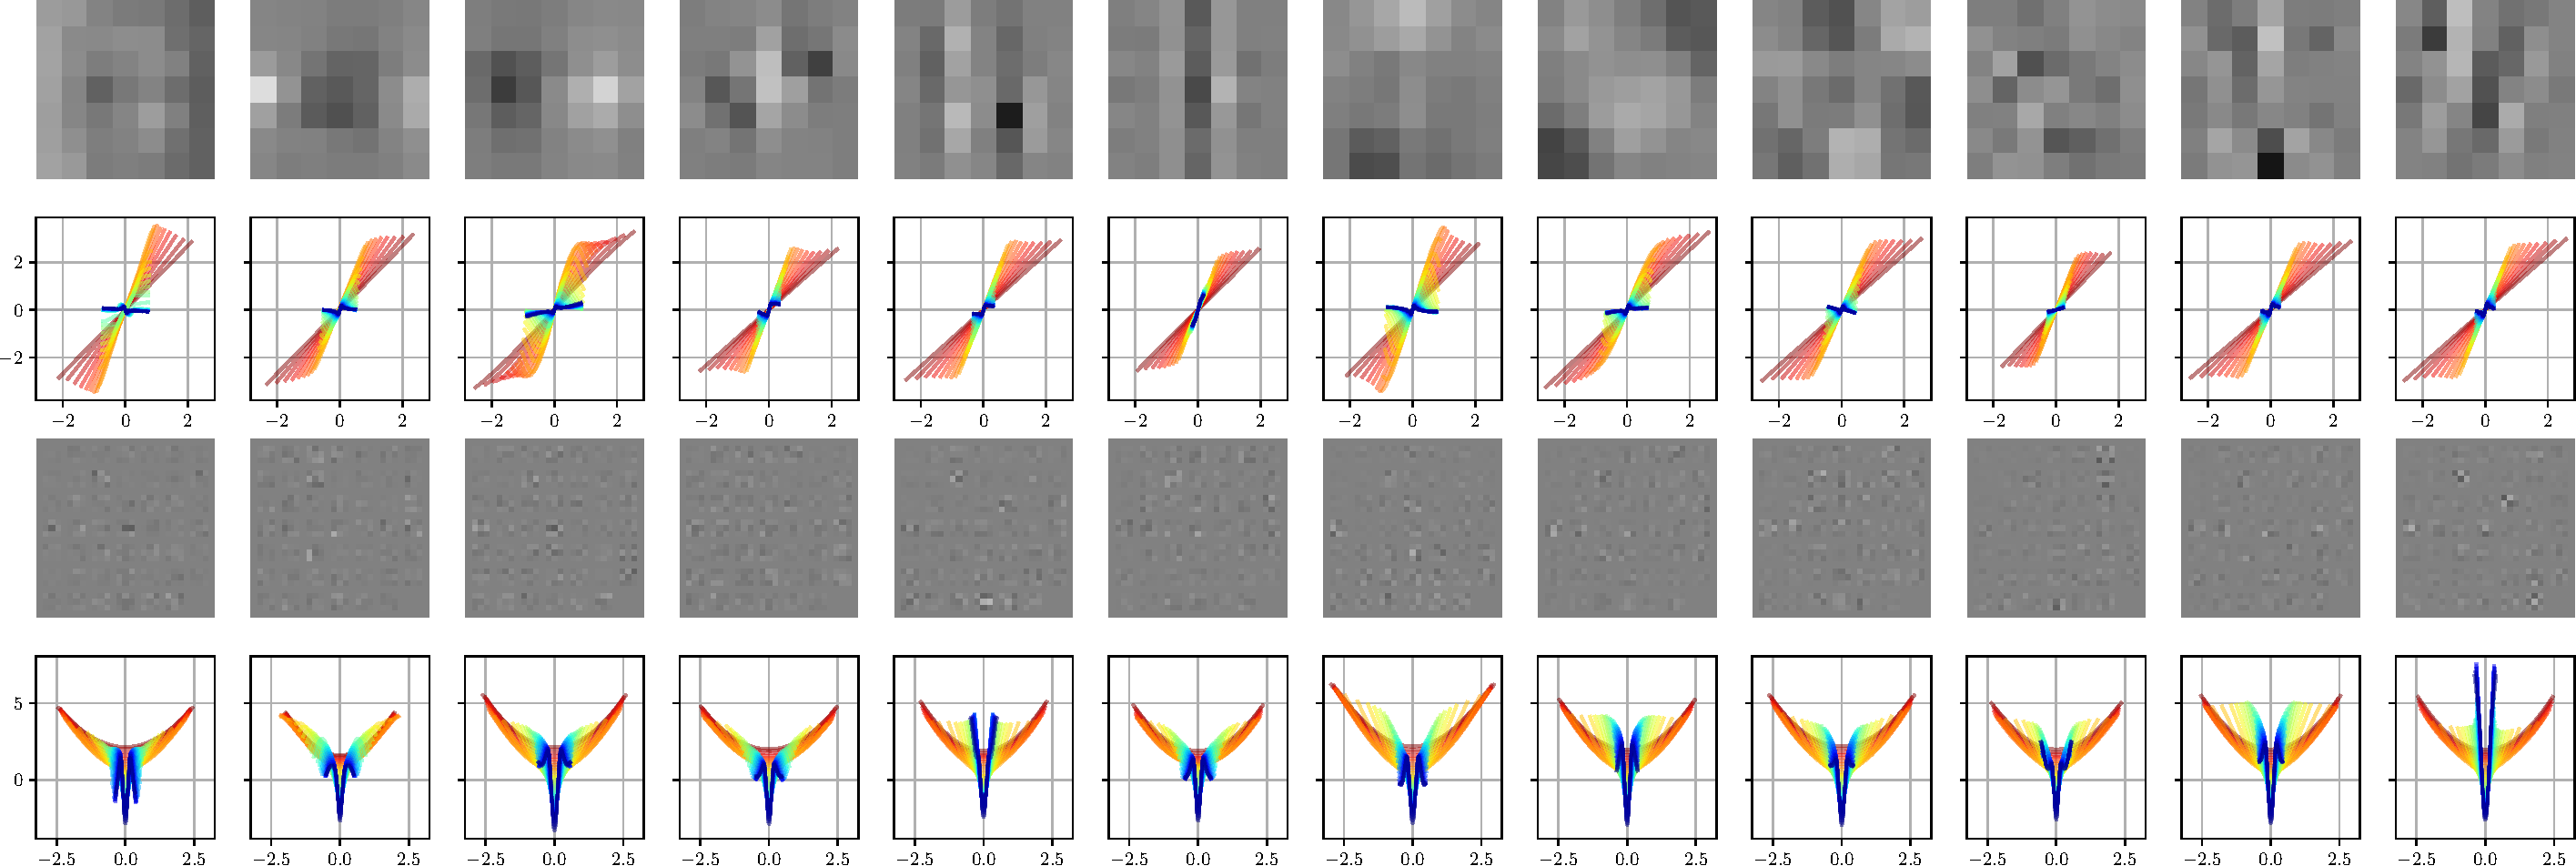
\includegraphics[width=.96\linewidth]{../figures/results/params_foedeep}};
\draw[black, very thick, rounded corners] (r2.north east) -- (r2.north west) -- (r2.south west) -- (r2.south east) node[midway,label,yshift=-1.25mm] {$R_2$};
\end{tikzpicture}
\end{center}
\begin{spacing}{1}
\LARGE
Illustration of convolution kernels and corresponding activation functions for a one-layer prior~$R_1$ (top) and two-layer prios~$R_2$ (bottom).
\end{spacing}

\section{Solving Inverse Problems using~$R_L$}
We aim at determining~$\rvx$ from an observation~$\rvz=A\rvx+\zeta$.
The maximum a posteriori estimator amounts to the variational approach\\[-1em]
% \vspace*{-10em}
% \begin{wrapfigure}{r}{.4\linewidth}
% \centering
% 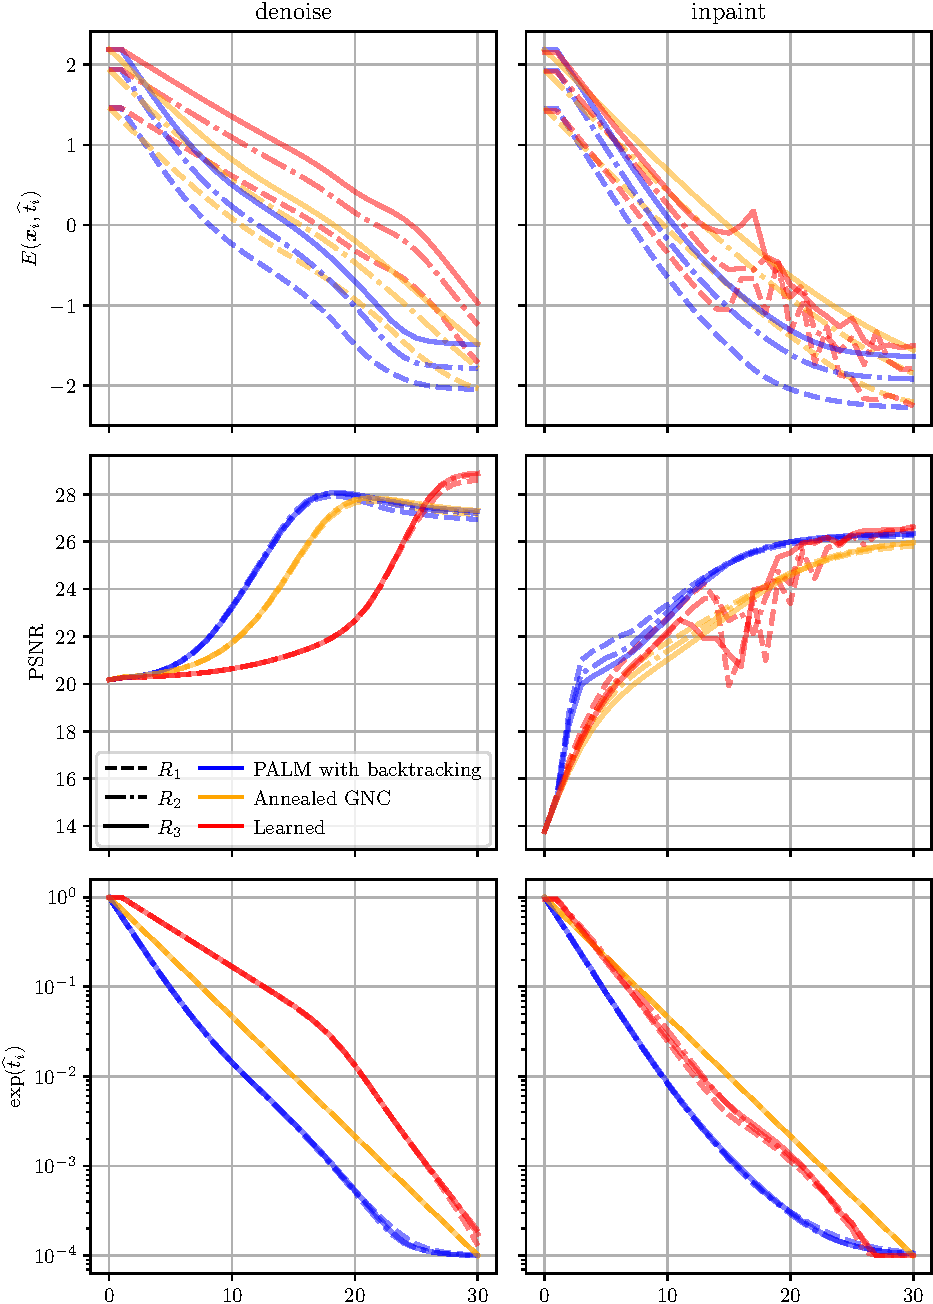
\includegraphics[width=.95\linewidth]{img/plots_denoise_inpaint}
% \end{wrapfigure}
\noindent\begin{minipage}[t]{.59\linewidth}
\vspace{0pt}
\[
\min_\vx\, R_L(\vx,\widehat{t}) + D(\vz,A\vx),
\]
% where~the data term~$D$ accounts for the noise characteristics of~$\zeta$.

\textbf{What about the additional $\widehat{t}$?}
\begin{itemize}
\item \emph{Joint optimization problem:} 
\[
\min_{\vx,\widehat{t}}\left\{R_L(\vx,\widehat{t}) + D(\vz,A\vx)\right\}
\]
can be efficiently solved using preconditioned proximal gradient descent.\\[-1.5ex]
\item \emph{Predefined schedule:}\\
graduated non-convexity heuristic or DDIM\\[-1.5ex]
\item \emph{Task-specific Learning of Schedule:}
\end{itemize}
\end{minipage}%
\hfill\begin{minipage}[t]{.4\linewidth}
\vspace{0pt}
    \begin{flushright}
        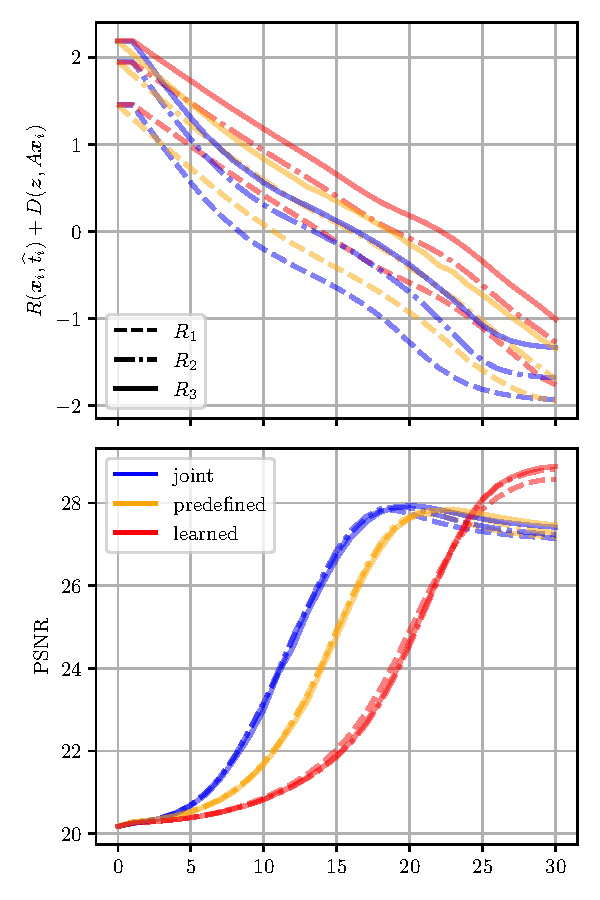
\includegraphics[width=.9\linewidth]{img/plots_denoise}
    \end{flushright}
\end{minipage}
\vspace*{1em}
\begin{itemize}
    \item[] This is \emph{equivalent to variational networks} and links them to diffusion-based models.
\end{itemize}
\columnbreak


\end{multicols}
}
% End of central box


% Bottom box with QR code
\bottombox{
    %% QR code
    % \qrcode{img/qrcode}{img/smartphoneWhite}{Scan QR code to get the full paper}
    % Comment out the line below out to hide logo
    % \hfill\bottomboxlogo{img/logo.eps} % \hfill shifts the logo across so it meets the right hand side margin
    % Note that \bottomboxlogo takes an optional width argument. It defaults to the following: 
    
\includegraphics[height=2.5cm]{img/ukb-logo.png} 
    \hfill
    
\includegraphics[height=2.5cm]{img/tug-logo.png} 
    % \bottomboxlogo[height=3cm]{img/tug-logo.png}
    % where \textwidth is actually the width of a minipage which is defined in the \bottombox command of
    % betterportaitposter.cls It's a standard \includegraphics command in there, so easy to change if 
    % you need to add a border etc.
}
% End of bottom box


%\qrcode{img/qrcode}{img/smartphoneWhite}{
%\textbf{Take a picture} to
%\\download the full paper
%}


%% Compact QR code (comment the previous command and uncomment this one to switch)
%\compactqrcode{img/qrcode}{
%\textbf{Take a picture} to
%\\download the full paper
%}

%}

\end{document}